\section{Étude des résultats}
    \paragraph{}Après avoir terminé la mise en place des algorithmes, nous avons procédé à une
    batterie de tests afin de déterminer le nombre d'itération et la durée de tabou les plus
    efficaces. Nous avons donc exécuté le programme plusieurs fois en alternant le nombre
    d'itération et la durée tabou entre les valeurs 5, 10, 15, 20 et 100.

    \paragraph{}Un fois les tests réalisés, dans on un premier temps on a cherché à définir le
    nombre d'itération le plus intéressant, c'est à dire un nombre suffisamment élevé pour permettre au
    projet de trouver une solution pertinente assez faible pour éviter au programme de tourner trop
    longtemps alors que la meilleur solution locale est obtenue.  
    \begin{center} 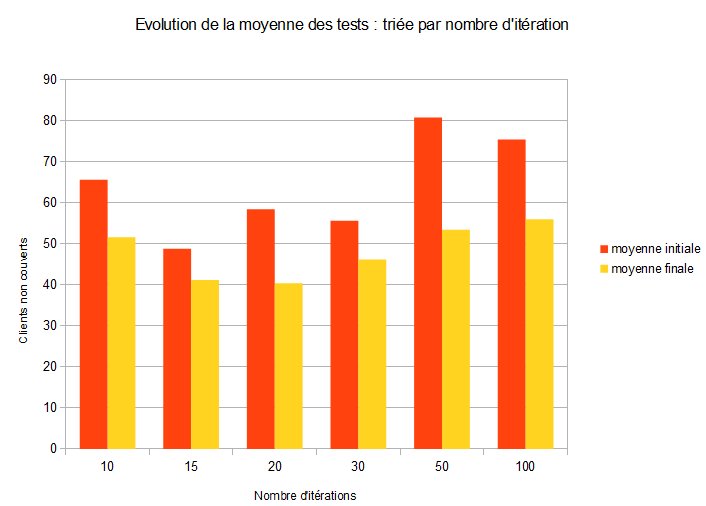
\includegraphics[scale=1]{ tableau_nombre_iteration } \end{center}
    \paragraph{} Suite à nos tests on peut constater que le plus grand écart entre les solutions
    initiales et les solutions finales apparait après 50 itération.

    \paragraph{}Dans un second temps, de la même manière on a cherché à optimisé la valeur de la
    durée tabou, on a donc procédé des tests afin de comparer les différentes valeurs.
    Une bonne durée tabou permet de retirer une solution durant une durée suffisante pour que le
    programme puisse s'éloigner de la solution actuelle pour chercher une nouvelle piste.
    \begin{center} 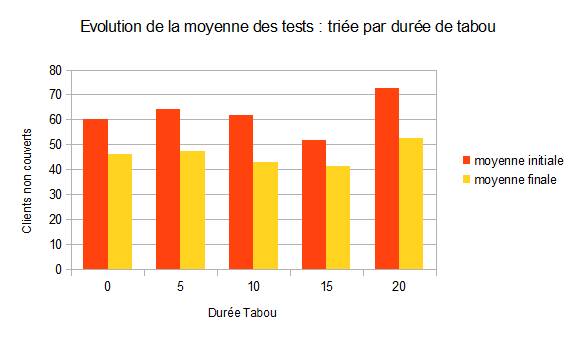
\includegraphics[scale=1]{tableau_duree_tabou} \end{center}
    \paragraph{}Suite à nos tests on constate que les valeurs les plus pertinentes sont 10 et 20,
    la différence jouant sur le nombre d'itération. Dans l'implémentation de notre solution la durée
    tabou nécessite d'être supérieur à 5 car pour chaque sites 3 permutations sont possible et si
    celle si ne varie pas ou peu l'algorithme restera bloquer sur un site sans visiter les autre
    solution. Une valeur de 10 à 20 permet au programme, dans les cas où les permutations sont
    égales, de visiter des solutions un peu plus éloigné.


    \paragraph{}Ensuite on a réuni nos résultats dans un même graphique afin de représenter les
    meilleurs solutions.
    \begin{center} 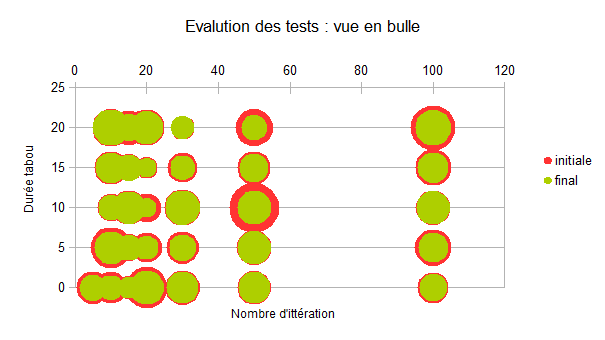
\includegraphics[scale=1]{tableau_bubulle} \end{center}
    \paragraph{}Le graphique confirme bien les résultats des précédents graphes, la solution avec 50
    itérations et une durée tabou de 10 est la plus efficace.

